% !TeX root = ../main.tex
% Add the above to each chapter to make compiling the PDF easier in some editors.

\chapter{Experimental Results}\label{chapter:results}

{\color{red} SOME INTRO SUMMARIZING THE FINDINGS IN BULLET POINTS}

We describe the complete experimental setups in Appendix \ref{appendix:experimental_setups}.

\section{Euclidean Flow Between Two Gaussians} \label{sec:gaussian_flow}

\begin{figure}[h!]
    \centering
    \begin{subfigure}{0.47\linewidth}
        \centering
        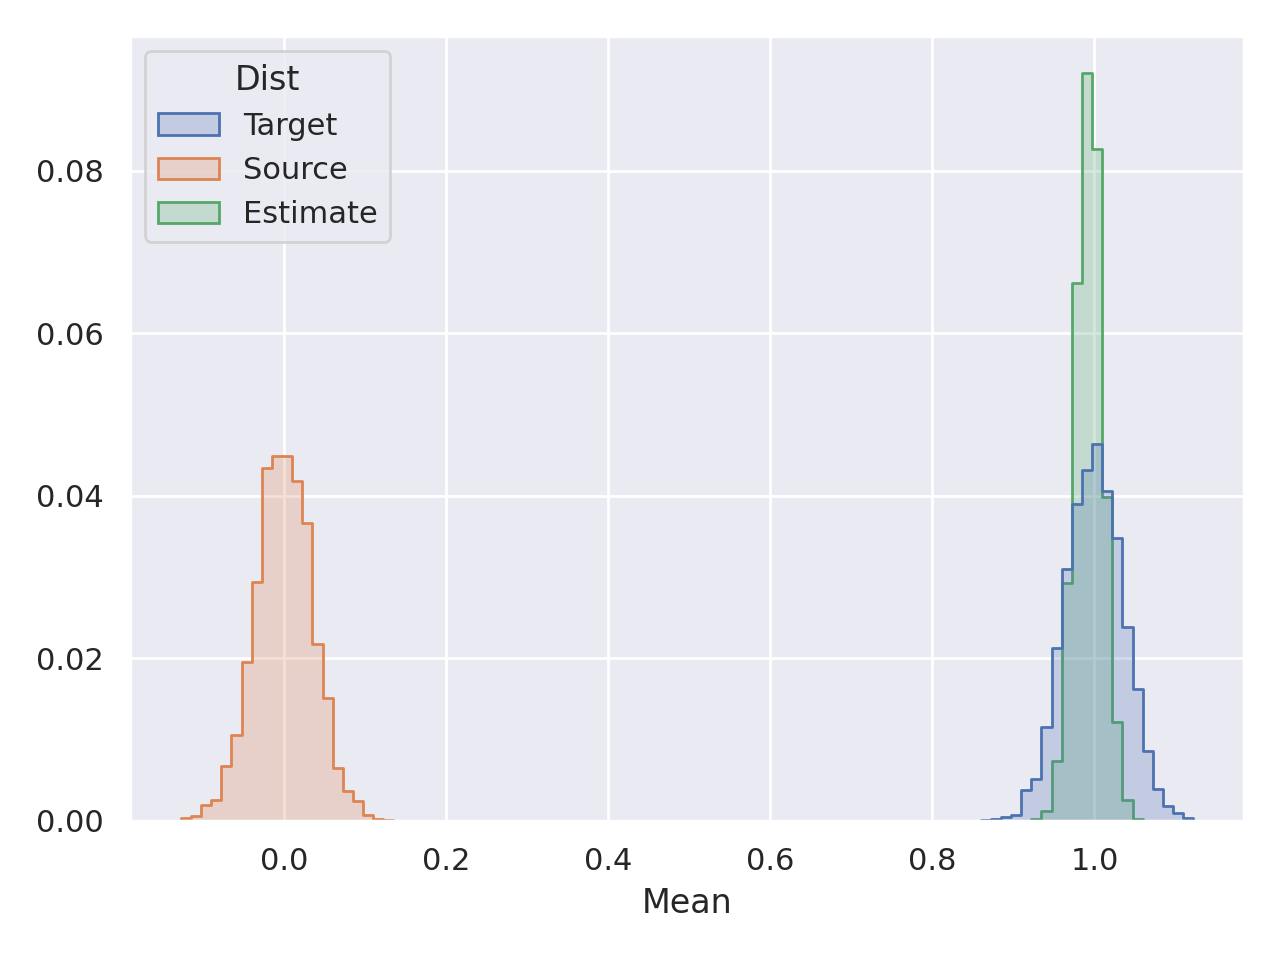
\includegraphics[width=\linewidth]{figures/gaussian/0.png}
        \caption{Deterministic sampling $(\varepsilon = 0)$}
        \label{fig:gaussian_deterministic}
    \end{subfigure}
    \begin{subfigure}{0.47\linewidth}
        \centering
        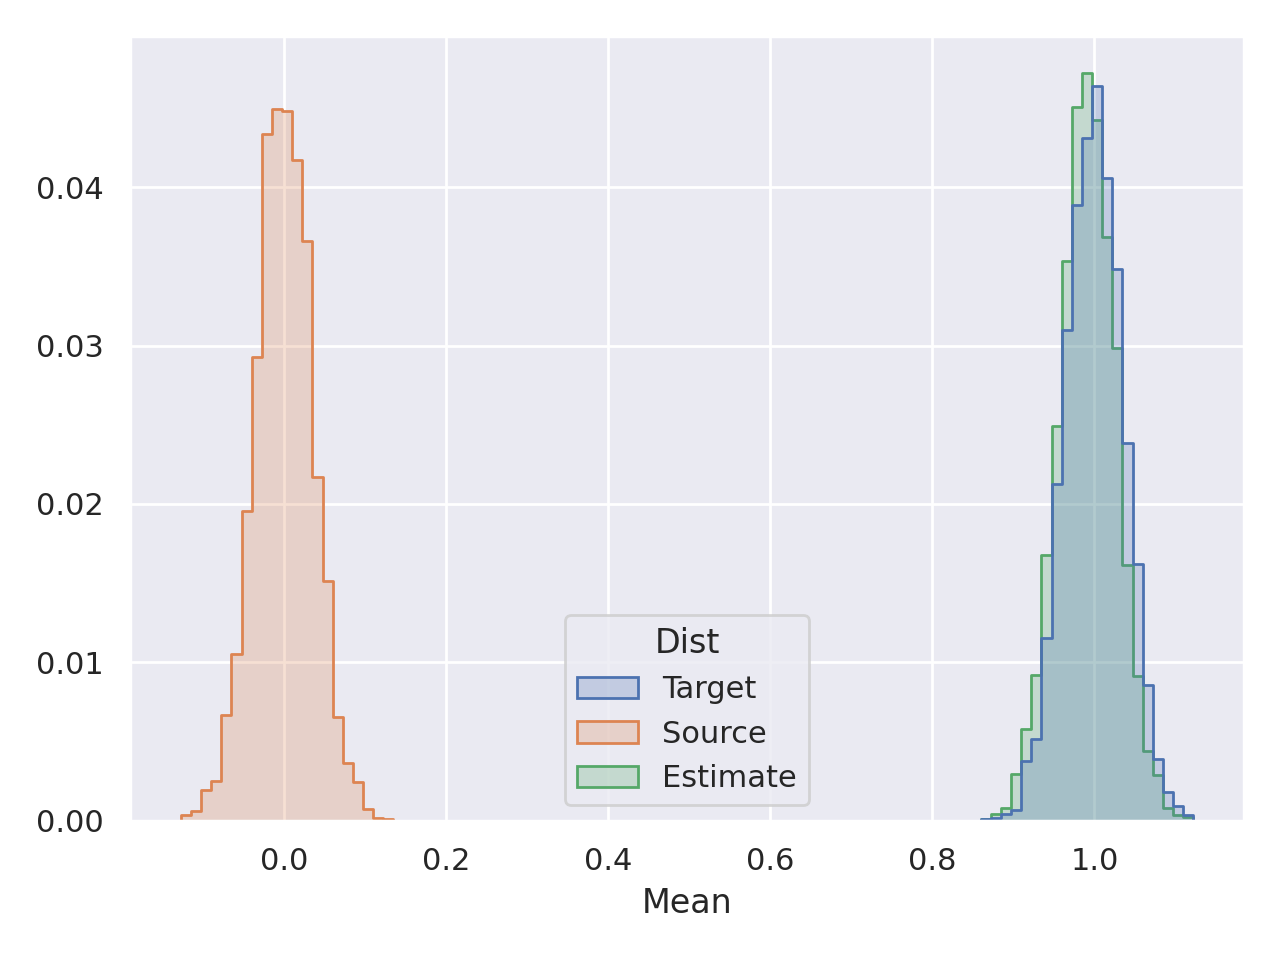
\includegraphics[width=\linewidth]{figures/gaussian/0.05.png}
        \caption{Stochastic sampling $(\varepsilon = 0.05)$}
        \label{fig:gaussian_stochastic}
    \end{subfigure}
    \caption{\label{fig:gaussian-results}\textbf{Histograms for the means of the weights generated by a Euclidean flow trained between two Gaussian distributions.} The flow fails to capture the variance in the target distribution with deterministic sampling, but this is corrected by stochastic sampling with $\varepsilon = 0.05$.} 
\end{figure}

To verify our approach of learning a flow model in weight-space, we begin our evaluation the toy task of learning a flow between two Gaussian distributions. The neural network is a small MLP with 30 input, two output dimensions, and two hidden layers of 16 neurons. We sample $X_0 \sim p_0 := \N(0, \mathbf{I})$ and $X_1 \sim p_1 := \N(1, \mathbf{I})$, and train our Euclidean flow to map $p_0$ to $p_1$ with independent coupling $q(x_0, x_1) = p_0(x_0)p_1(x_1)$. This is a relatively simpler task than learning over actual weights since each weight is sampled independently. 

Figure \ref{fig:gaussian-results} shows histograms of the means of the weights sampled from the flow with 100 Euler steps, and either deterministic or stochastic $(\varepsilon=0.05)$ sampling. Independent of the sampling method used, the flow covers the high-density center of the target distribution well, but the weights sampled deterministically fail to capture the variance in the target distribution. Stochastic sampling however appears to correct for this over-saturation and leads to more diverse samples. Overall, these results validates the feasability of learning a flow model in weight-space using graph neural networks, and we move on to tasks involving actual learned weights. 


\section{Classification with a Small Model}

Describe the model as well, mention why we can go geometric since relu activations. 

\begin{table}[h!]
    \centering
    \begin{tabular}{lll}
        \toprule
        \textbf{Flow}  & \textbf{Accuracy} & \textbf{Loss} \\
        \midrule
        Euclidean  & 0.998 ± 0.006 & 0.101 ± 0.05 \\ 
        Euclidean (aligned)  & 0.998 ± 0.006 & 0.07 ± 0.04 \\
        \midrule
        Normalized  & 0.993 ± 0.009 & 0.027 ± 0.014 \\
        Normalized (aligned)  & 0.989 ± 0.011 & 0.03 ± 0.015 \\
        \midrule
        Geometric  & 0.815 ± 0.279 & 0.525 ± 0.81 \\
        Geometric (aligned)  & 0.819 ± 0.277 & 0.551 ± 0.872 \\
        \midrule
        \textbf{Target} & 0.992 ± 0.01 & 0.048 ± 0.032 \\
        \bottomrule
    \end{tabular}
    \caption{\label{tab:uci_class_table}UCI results direct sample quality}
\end{table}

\begin{figure}[h!]
    \centering
    \begin{subfigure}{0.47\linewidth}
        \centering
        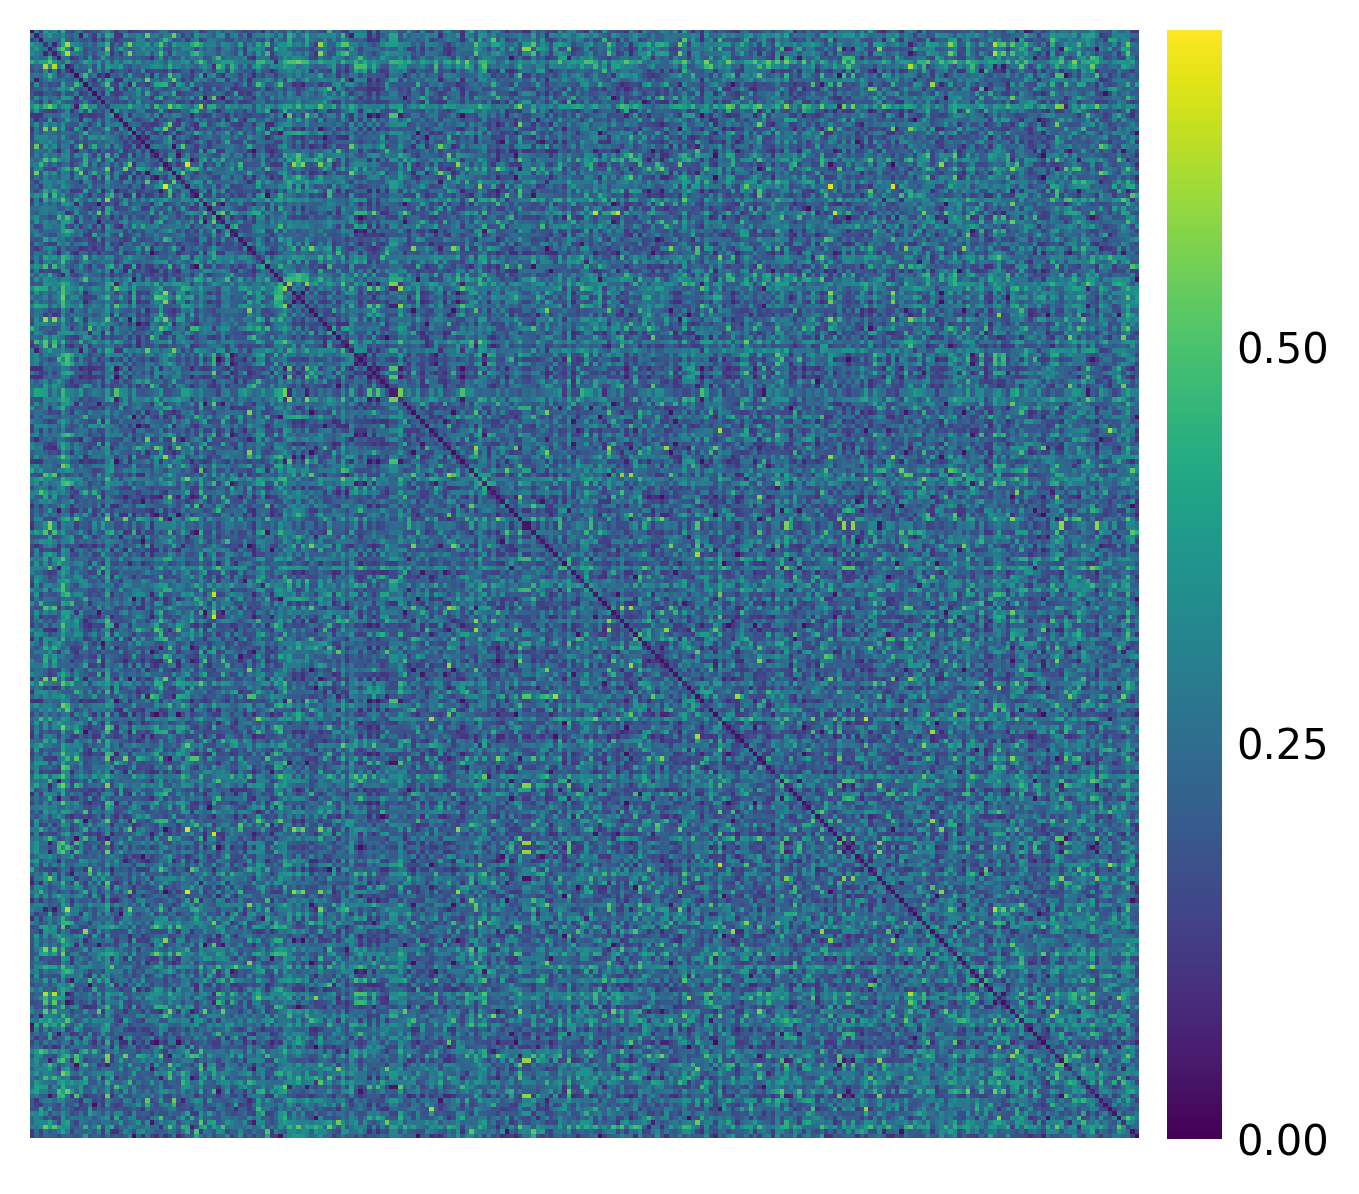
\includegraphics[width=\linewidth]{figures/uci_17/uci_17_unaligned.png}
        \caption{Unaligned (0.244 ± 0.009)}
        \label{fig:uci_unaligned}
    \end{subfigure}
    \begin{subfigure}{0.47\linewidth}
        \centering
        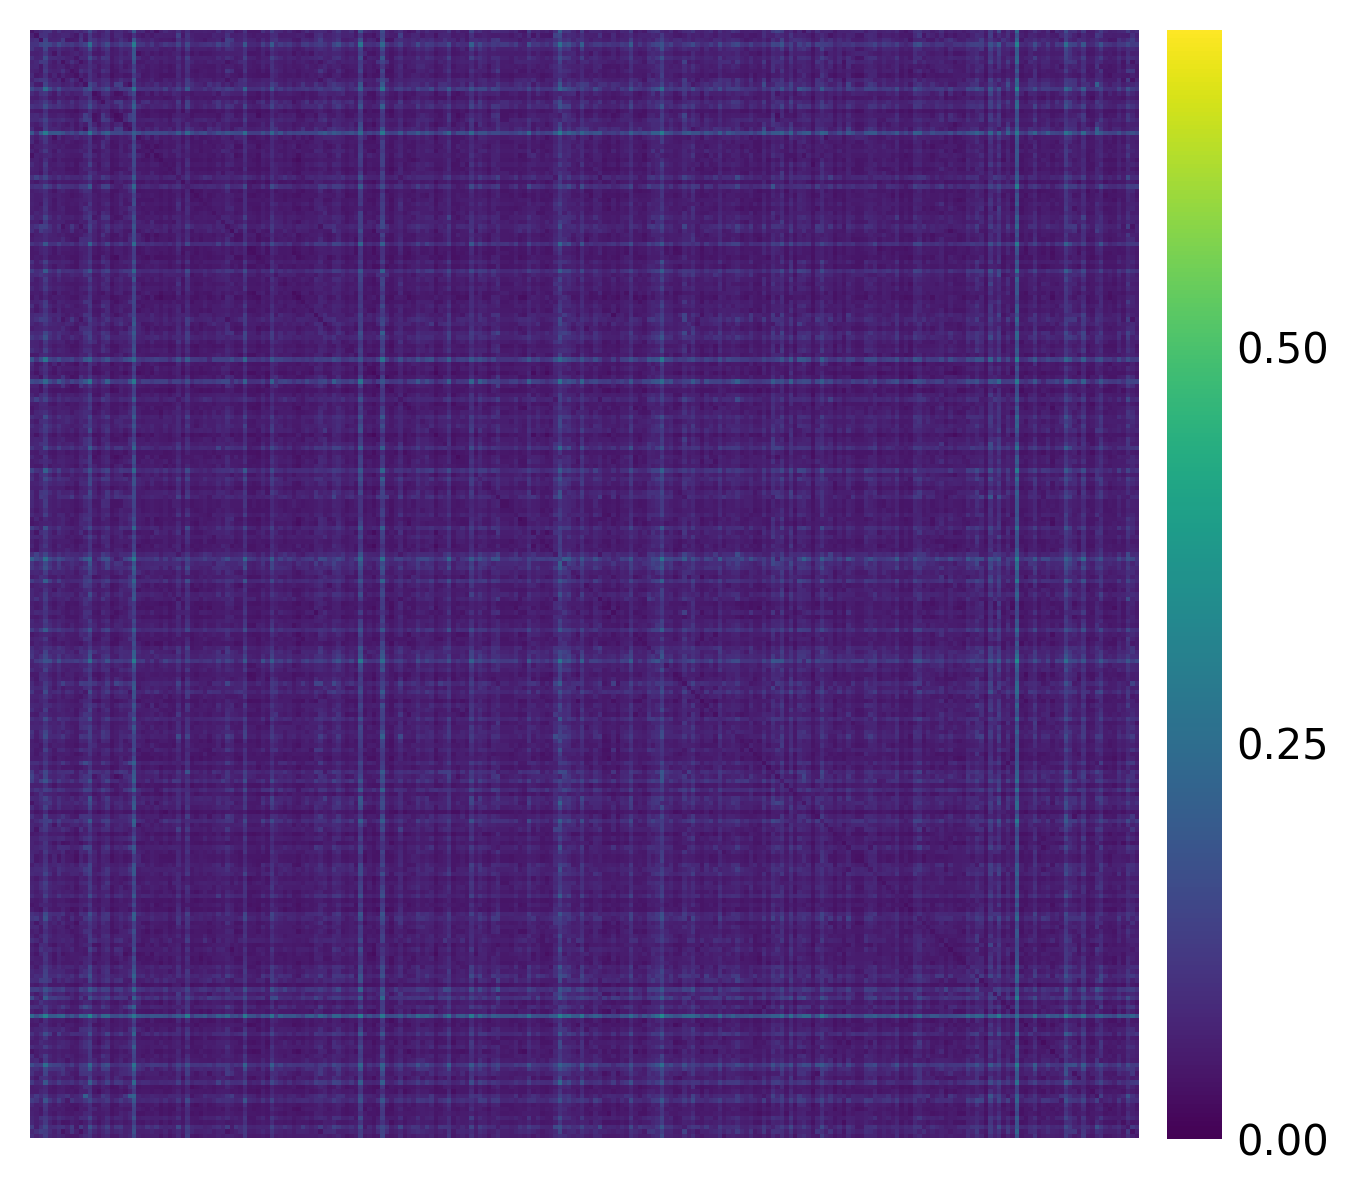
\includegraphics[width=\linewidth]{figures/uci_17/uci_17_aligned.png}
        \caption{Aligned (0.070 ± 0.001)}
        \label{fig:uci_aligned}
    \end{subfigure}
    \caption{\label{fig:uci_alignment}\textbf{Loss barriers for 250 weights across different optimization trajectories} (mean and standard deviations in parentheses). Aligning all weights to a single reference significantly reduces the loss barriers between the weights. } 
\end{figure}




{\color{orange} how this task is easy since convex after alignment etc etc, but need to show with results}